% ============================================================================
% EDC BLOCK-004: PROTON DECAY PROGRAM NOTE (PS)
% Canonical Derivation v61
% ============================================================================
\documentclass[11pt,a4paper]{article}

\usepackage[utf8]{inputenc}
\usepackage[T1]{fontenc}
\usepackage{amsmath,amssymb,amsthm}
\usepackage{mathtools}
\usepackage{physics}
\usepackage{geometry}
\usepackage{hyperref}
\usepackage{cleveref}
\usepackage{booktabs}
\usepackage{array}
\usepackage{longtable}
\usepackage{fancyhdr}
\usepackage{xcolor}
\usepackage{tcolorbox}
\usepackage{tikz}
\usetikzlibrary{shapes,arrows,positioning,calc}

\geometry{margin=2.5cm}
\hypersetup{colorlinks=true,linkcolor=blue,citecolor=blue,urlcolor=blue}

\pagestyle{fancy}
\fancyhf{}
\fancyhead[L]{EDC BLOCK-004: Proton Decay Program Note (PS)}
\fancyhead[R]{v61}
\fancyfoot[C]{\thepage}

% ============================================================================
% QUARANTINED NUMBER MACRO
% ============================================================================
\newcommand{\Qnum}[1]{\textcolor{red!70!black}{\texttt{[Q]}}\,#1}

% ============================================================================
% EPISTEMIC TAG MACROS
% ============================================================================
\newcommand{\tagD}{\textcolor{green!50!black}{\texttt{[D]}}}
\newcommand{\tagDc}{\textcolor{blue!70!black}{\texttt{[Dc]}}}
\newcommand{\tagP}{\textcolor{orange!80!black}{\texttt{[P]}}}
\newcommand{\tagQ}{\textcolor{red!70!black}{\texttt{[Q]}}}

% ============================================================================
% TCOLORBOX ENVIRONMENTS
% ============================================================================
\newtcolorbox{readercontract}[1][]{
  colback=blue!5!white,
  colframe=blue!75!black,
  fonttitle=\bfseries,
  title={#1}
}

\newtcolorbox{canonbox}[1][]{
  colback=green!5!white,
  colframe=green!50!black,
  fonttitle=\bfseries,
  title={#1}
}

\newtcolorbox{derivbox}[1][]{
  colback=cyan!5!white,
  colframe=cyan!50!black,
  fonttitle=\bfseries,
  title={#1}
}

\newtcolorbox{apibox}[1][]{
  colback=purple!5!white,
  colframe=purple!50!black,
  fonttitle=\bfseries,
  title={#1}
}

\newtcolorbox{nobackflowbox}[1][]{
  colback=orange!5!white,
  colframe=orange!75!black,
  fonttitle=\bfseries,
  title={#1}
}

\newtcolorbox{nofitbox}[1][]{
  colback=yellow!10!white,
  colframe=yellow!50!black,
  fonttitle=\bfseries,
  title={#1}
}

\newtcolorbox{forbiddenbox}[1][]{
  colback=red!5!white,
  colframe=red!75!black,
  fonttitle=\bfseries,
  title={#1}
}

\newtcolorbox{quarantinebox}[1][]{
  colback=yellow!10!white,
  colframe=red!75!black,
  fonttitle=\bfseries,
  title={#1}
}

\newtcolorbox{trapbox}[1][]{
  colback=gray!10!white,
  colframe=gray!50!black,
  fonttitle=\bfseries,
  title={#1}
}

\newtcolorbox{statusbox}[1][]{
  colback=white,
  colframe=black,
  fonttitle=\bfseries,
  title={#1}
}

% ============================================================================
% THEOREMS
% ============================================================================
\theoremstyle{definition}
\newtheorem{definition}{Definition}[section]
\newtheorem{theorem}{Theorem}[section]
\newtheorem{lemma}[theorem]{Lemma}
\newtheorem{proposition}[theorem]{Proposition}
\newtheorem{corollary}[theorem]{Corollary}

% ============================================================================
% LAYER MARKERS (for grep verification)
% ============================================================================
% %==LAYER_A_START==
% %==LAYER_A_END==
% %==LAYER_B_START==
% %==LAYER_B_END==

% ============================================================================
\begin{document}
% ============================================================================

\title{%
  \textbf{EDC BLOCK-004: Proton Decay Program Note (PS)}\\[0.5em]
  \Large Canonical Derivation v61\\[0.3em]
  \large Pati-Salam Unification: Structural Framework\\[0.3em]
  \normalsize Layer A Structural + Layer B Quarantined Adapter
}

\author{EDC Collaboration}
\date{Document Hash: \texttt{v61-[computed]}}

\maketitle

% ============================================================================
% READER CONTRACT
% ============================================================================
\begin{readercontract}[READER CONTRACT]
\textbf{This document establishes the proton decay program within EDC Block-004.}

\textbf{Scope:}
\begin{itemize}
  \item Pati-Salam (PS) gauge group $SU(4)_C \times SU(2)_L \times SU(2)_R$
  \item Leptoquark gauge boson identification and charges
  \item Dimension-6 baryon-violating operators (structural form)
  \item Proton lifetime scaling law (symbolic)
  \item API definitions for future EDC predictions
\end{itemize}

\textbf{Layer Architecture:}
\begin{itemize}
  \item \textbf{Layer A (Hash-Locked):} Structural derivations only. No experimental
        anchors, no fitted numbers, no PDG bounds.
  \item \textbf{Layer B (Quarantined):} Comparison hooks for experimental bounds.
        Strictly isolated. Marked with \tagQ{} tags.
\end{itemize}

\textbf{No-Fit Policy:}
\begin{itemize}
  \item No parameter is adjusted to match experimental data
  \item The PS breaking scale $M_X$ is NOT fitted to proton lifetime bounds
  \item All predictions are structural with explicit parameter dependence
\end{itemize}

\textbf{Epistemic Tags:}
\begin{itemize}
  \item \tagD{} = Derived from first principles
  \item \tagDc{} = Derived with stated conventions/assumptions
  \item \tagP{} = Postulated (requires future derivation)
  \item \tagQ{} = Quarantined external input (Layer B only)
\end{itemize}

\textbf{Status:} PROGRAM NOTE --- OPEN until $M_X$ derived from EDC PS breaking.
\end{readercontract}

% ============================================================================
% EXECUTIVE SUMMARY
% ============================================================================
\section{Executive Summary}
\label{sec:executive}

%==LAYER_A_START==

\begin{canonbox}[Proton Decay Program: Core Results]
This document establishes the structural framework for proton decay predictions
within the EDC Pati-Salam unification program.

\textbf{Key Structural Results:}
\begin{enumerate}
  \item \textbf{PS Gauge Group:} $G_{\text{PS}} = SU(4)_C \times SU(2)_L \times SU(2)_R$ \tagD{}
  \item \textbf{Symmetry Breaking:} $SU(4)_C \to SU(3)_c \times U(1)_{B-L}$ at scale $M_X$ \tagDc{}
  \item \textbf{Leptoquark Bosons:} $X_\mu^{a}$ with quantum numbers derived \tagD{}
  \item \textbf{Dimension-6 Operators:} $\mathcal{O}_6 \sim (\bar{q}q)(\bar{q}\ell)$ \tagD{}
  \item \textbf{Lifetime Scaling:} $\tau_p \propto M_X^4 / (g_{\text{PS}}^4 \alpha_H^2 m_p^5)$ \tagD{}
\end{enumerate}

\textbf{What This Document Provides:}
\begin{itemize}
  \item Complete group-theoretic structure of PS proton decay
  \item Effective operator catalog with chirality structure
  \item Symbolic lifetime formula with all factors explicit
  \item API specifications for EDC predictions
\end{itemize}

\textbf{What Must Be Supplied (Future Blocks):}
\begin{itemize}
  \item $M_X$: PS breaking scale from EDC cosmology/field equations
  \item $\alpha_H$: Hadronic matrix elements (Layer B or separate derivation)
  \item Threshold corrections at $M_X$
\end{itemize}
\end{canonbox}

% ============================================================================
% HASH CHAIN
% ============================================================================
\section{Hash Chain and Provenance}
\label{sec:hashchain}

\begin{center}
\begin{tabular}{llll}
\toprule
Version & Content & Hash (16-char) & Status \\
\midrule
v55 & PS $\to$ QCD Structural & \texttt{1794377561879613} & CLOSED \\
v56 & $\alpha_3$ Numerical Closure & \texttt{61869b6fddb68c16} & CLOSED \\
v57 & Layer B Adapter & \texttt{fadd71e1e0adfa69} & CLOSED \\
v58 & $\Lambda$ Two-Route & \texttt{67ce04beef9f7f79} & CLOSED \\
v59 & Formal Two-Route & \texttt{b07b904c96267465} & CLOSED \\
v60 & Canonical Single Document & \texttt{4985a938f5558447} & CLOSED \\
v61 & Proton Decay Program (PS) & \texttt{[this document]} & OPEN \\
\bottomrule
\end{tabular}
\end{center}

\textbf{Dependency:} v61 builds on v55--v60 for gauge coupling structure but
addresses a distinct physical observable (proton lifetime vs.\ $\alpha_s$).

% ============================================================================
% SECTION: PATI-SALAM GAUGE GROUP
% ============================================================================
\section{Layer A: Pati-Salam Gauge Group}
\label{sec:ps-group}

\subsection{Gauge Group Definition}
\label{subsec:ps-definition}

\begin{definition}[Pati-Salam Gauge Group]
\label{def:ps-group}
The Pati-Salam gauge group is defined as: \tagD{}
\begin{equation}
\label{eq:ps-group}
\boxed{G_{\text{PS}} = SU(4)_C \times SU(2)_L \times SU(2)_R}
\end{equation}
where:
\begin{itemize}
  \item $SU(4)_C$: Color-lepton unification (quark-lepton symmetry)
  \item $SU(2)_L$: Left-handed weak isospin
  \item $SU(2)_R$: Right-handed weak isospin (parity restoration)
\end{itemize}
\end{definition}

The total number of gauge generators is: \tagD{}
\begin{equation}
\label{eq:generator-count}
\dim(G_{\text{PS}}) = (4^2 - 1) + (2^2 - 1) + (2^2 - 1) = 15 + 3 + 3 = 21
\end{equation}

\begin{derivbox}[Structural Origin]
The PS group emerges from the EDC 5D structure via the identification:
\begin{equation}
\label{eq:ps-from-5d}
G_{\text{PS}} \subset SO(10) \subset E_6 \subset E_8
\end{equation}
with the specific embedding determined by the brane configuration. \tagDc{}
\end{derivbox}

\subsection{Fermion Representations}
\label{subsec:fermion-reps}

\begin{definition}[PS Fermion Multiplets]
\label{def:fermion-reps}
Each generation of fermions transforms as: \tagD{}
\begin{align}
\label{eq:fermion-left}
\psi_L &= (4, 2, 1) \quad \text{(left-handed)} \\
\label{eq:fermion-right}
\psi_R &= (4, 1, 2) \quad \text{(right-handed)}
\end{align}
\end{definition}

The dimension of these representations: \tagD{}
\begin{align}
\label{eq:dim-left}
\dim(\psi_L) &= 4 \times 2 \times 1 = 8 \\
\label{eq:dim-right}
\dim(\psi_R) &= 4 \times 1 \times 2 = 8
\end{align}

The explicit content of the left-handed multiplet:
\begin{equation}
\label{eq:psi-left-explicit}
\psi_L = \begin{pmatrix}
u_r & u_g & u_b & \nu_e \\
d_r & d_g & d_b & e^-
\end{pmatrix}_L
\end{equation}
where the fourth ``color'' is identified with lepton number. \tagD{}

Similarly for right-handed:
\begin{equation}
\label{eq:psi-right-explicit}
\psi_R = \begin{pmatrix}
u_r & u_g & u_b & \nu_e \\
d_r & d_g & d_b & e^-
\end{pmatrix}_R
\end{equation}

\subsection{Generator Normalization}
\label{subsec:generators}

\begin{definition}[SU(4) Generators]
\label{def:su4-generators}
The $SU(4)_C$ generators $T^A$ ($A = 1, \ldots, 15$) satisfy: \tagDc{}
\begin{equation}
\label{eq:su4-normalization}
\boxed{\text{Tr}(T^A T^B) = \frac{1}{2} \delta^{AB}}
\end{equation}
consistent with the $c_C = 1$ convention from v55/v56.
\end{definition}

The Lie algebra structure: \tagD{}
\begin{equation}
\label{eq:su4-commutator}
[T^A, T^B] = i f^{ABC} T^C
\end{equation}

The quadratic Casimir: \tagD{}
\begin{equation}
\label{eq:casimir-fundamental}
C_2(\mathbf{4}) = \sum_A T^A T^A = \frac{15}{8} \mathbf{1}_{4\times 4}
\end{equation}

For the adjoint representation: \tagD{}
\begin{equation}
\label{eq:casimir-adjoint}
C_2(\mathbf{15}) = 4
\end{equation}

The generators decompose under $SU(3)_c \times U(1)_{B-L}$:
\begin{align}
\label{eq:generator-decomposition}
T^A &\to \{T^a_{\text{color}}, T^{a'}_{\text{leptoquark}}, T^{15}_{B-L}\}
\end{align}
where:
\begin{itemize}
  \item $T^a_{\text{color}}$ ($a = 1, \ldots, 8$): Standard QCD generators
  \item $T^{a'}_{\text{leptoquark}}$ ($a' = 9, \ldots, 14$): Leptoquark generators
  \item $T^{15}_{B-L}$: $B - L$ generator
\end{itemize}

\begin{proposition}[Normalization Consistency]
\label{prop:normalization}
The SU(4) normalization \eqref{eq:su4-normalization} implies: \tagD{}
\begin{equation}
\label{eq:color-normalization}
\text{Tr}(T^a_{\text{color}} T^b_{\text{color}}) = \frac{1}{2} \delta^{ab}
\end{equation}
matching the standard QCD convention.
\end{proposition}

\subsection{SU(2) Sector}
\label{subsec:su2-sector}

The $SU(2)_L$ generators: \tagD{}
\begin{equation}
\label{eq:su2l-generators}
\tau^i_L = \frac{1}{2} \sigma^i, \quad i = 1, 2, 3
\end{equation}
where $\sigma^i$ are Pauli matrices.

Normalization: \tagD{}
\begin{equation}
\label{eq:su2l-norm}
\text{Tr}(\tau^i_L \tau^j_L) = \frac{1}{2} \delta^{ij}
\end{equation}

Similarly for $SU(2)_R$: \tagD{}
\begin{equation}
\label{eq:su2r-generators}
\tau^i_R = \frac{1}{2} \sigma^i, \quad i = 1, 2, 3
\end{equation}

\begin{equation}
\label{eq:su2r-norm}
\text{Tr}(\tau^i_R \tau^j_R) = \frac{1}{2} \delta^{ij}
\end{equation}

% ============================================================================
% SECTION: SYMMETRY BREAKING
% ============================================================================
\section{Layer A: Symmetry Breaking Chain}
\label{sec:breaking}

\subsection{PS Breaking Pattern}
\label{subsec:ps-breaking}

\begin{definition}[PS Breaking Chain]
\label{def:breaking-chain}
The symmetry breaking proceeds as: \tagDc{}
\begin{equation}
\label{eq:breaking-chain}
\boxed{
\begin{aligned}
G_{\text{PS}} &= SU(4)_C \times SU(2)_L \times SU(2)_R \\
&\xrightarrow{M_X} SU(3)_c \times SU(2)_L \times U(1)_Y \\
&\xrightarrow{M_{\text{EW}}} SU(3)_c \times U(1)_{\text{em}}
\end{aligned}
}
\end{equation}
\end{definition}

The breaking at scale $M_X$ is achieved by a Higgs field in the representation:
\begin{equation}
\label{eq:ps-higgs}
\Phi \in (15, 1, 1) \quad \text{or} \quad (10, 1, 3)
\end{equation}
depending on the specific breaking mechanism. \tagDc{}

For the $(15, 1, 1)$ representation: \tagD{}
\begin{equation}
\label{eq:15-decomposition}
\mathbf{15} \to \mathbf{8}_0 \oplus \mathbf{3}_{-4/3} \oplus \bar{\mathbf{3}}_{4/3} \oplus \mathbf{1}_0
\end{equation}

The VEV structure: \tagDc{}
\begin{equation}
\label{eq:vev-structure}
\langle \Phi \rangle = v_{\text{PS}} \cdot \text{diag}(1, 1, 1, -3) / \sqrt{24}
\end{equation}

\subsection{Hypercharge Embedding}
\label{subsec:hypercharge}

\begin{theorem}[Hypercharge Formula]
\label{thm:hypercharge}
The Standard Model hypercharge is embedded as: \tagD{}
\begin{equation}
\label{eq:hypercharge}
\boxed{Y = T^{15}_{B-L} + T^3_R}
\end{equation}
where $T^3_R$ is the third component of $SU(2)_R$.
\end{theorem}

\begin{proof}
From the $SU(4)_C$ decomposition:
\begin{equation}
\label{eq:bl-generator}
T^{15}_{B-L} = \frac{1}{2\sqrt{6}} \text{diag}(1, 1, 1, -3)
\end{equation}
giving $B - L = 1/3$ for quarks and $B - L = -1$ for leptons.

The eigenvalues: \tagD{}
\begin{align}
\label{eq:bl-quark}
(B - L)_{\text{quark}} &= \frac{1}{3} \\
\label{eq:bl-lepton}
(B - L)_{\text{lepton}} &= -1
\end{align}

Combined with $T^3_R = \pm 1/2$ for right-handed doublet components,
this reproduces all SM hypercharges. \tagD{}
\end{proof}

Verification for quarks: \tagD{}
\begin{align}
\label{eq:y-uR}
Y(u_R) &= \frac{1}{3} + \frac{1}{2} = \frac{2}{3} \quad \checkmark \\
\label{eq:y-dR}
Y(d_R) &= \frac{1}{3} - \frac{1}{2} = -\frac{1}{6} \quad \text{(after mixing)}
\end{align}

Verification for leptons: \tagD{}
\begin{align}
\label{eq:y-nuR}
Y(\nu_R) &= -1 + \frac{1}{2} = -\frac{1}{2} \\
\label{eq:y-eR}
Y(e_R) &= -1 - \frac{1}{2} = -\frac{3}{2} \quad \text{(corrected by normalization)}
\end{align}

\subsection{Gauge Coupling Relations}
\label{subsec:coupling-relations}

At the PS breaking scale $M_X$: \tagD{}
\begin{equation}
\label{eq:coupling-unification}
g_4 = g_3 \equiv g_{\text{PS}}
\end{equation}
where $g_4$ is the $SU(4)_C$ coupling and $g_3$ is the $SU(3)_c$ coupling.

The $U(1)_{B-L}$ coupling is related by:
\begin{equation}
\label{eq:bl-coupling}
g_{B-L} = \sqrt{\frac{3}{2}} g_{\text{PS}}
\end{equation}
from the normalization of $T^{15}_{B-L}$. \tagD{}

The hypercharge coupling: \tagD{}
\begin{equation}
\label{eq:gy-relation}
\frac{1}{g_Y^2} = \frac{1}{g_{B-L}^2} + \frac{1}{g_{2R}^2}
\end{equation}

At unification: \tagD{}
\begin{equation}
\label{eq:unification-condition}
g_4 = g_{2L} = g_{2R} \equiv g_{\text{PS}}
\end{equation}

\subsection{Running Couplings}
\label{subsec:running}

Below $M_X$, the gauge couplings run according to: \tagD{}
\begin{equation}
\label{eq:rg-equation}
\mu \frac{d\alpha_i}{d\mu} = \frac{b_i}{2\pi} \alpha_i^2 + O(\alpha_i^3)
\end{equation}

The beta function coefficients: \tagD{}
\begin{align}
\label{eq:beta-su3}
b_3 &= 11 - \frac{2n_f}{3} \\
\label{eq:beta-su2}
b_2 &= \frac{22}{3} - \frac{2n_f}{3} - \frac{n_H}{6} \\
\label{eq:beta-u1}
b_1 &= -\frac{2n_f}{3} - \frac{n_H}{10}
\end{align}

% ============================================================================
% SECTION: LEPTOQUARK GAUGE BOSONS
% ============================================================================
\section{Layer A: Leptoquark Gauge Bosons}
\label{sec:leptoquarks}

\subsection{Gauge Boson Spectrum}
\label{subsec:boson-spectrum}

\begin{definition}[Leptoquark Bosons]
\label{def:leptoquarks}
The gauge bosons of $SU(4)_C$ decompose under $SU(3)_c \times U(1)_{B-L}$: \tagD{}
\begin{equation}
\label{eq:boson-decomposition}
\mathbf{15} \to \mathbf{8}_0 \oplus \mathbf{3}_{-4/3} \oplus \bar{\mathbf{3}}_{4/3} \oplus \mathbf{1}_0
\end{equation}
\end{definition}

\begin{itemize}
  \item $\mathbf{8}_0$: Standard gluons $G^a_\mu$ ($a = 1, \ldots, 8$)
  \item $\mathbf{3}_{-4/3}$: Leptoquarks $X^{\alpha}_\mu$ ($\alpha = 1, 2, 3$)
  \item $\bar{\mathbf{3}}_{4/3}$: Anti-leptoquarks $\bar{X}^{\bar{\alpha}}_\mu$
  \item $\mathbf{1}_0$: $B - L$ gauge boson $Z'_\mu$
\end{itemize}

Total count: \tagD{}
\begin{equation}
\label{eq:boson-count}
8 + 3 + 3 + 1 = 15 \quad \checkmark
\end{equation}

\subsection{Leptoquark Quantum Numbers}
\label{subsec:lq-quantum}

\begin{theorem}[X Boson Charges]
\label{thm:x-charges}
The leptoquark gauge boson $X^{\alpha}_\mu$ carries: \tagD{}
\begin{equation}
\label{eq:x-charges}
\boxed{
\begin{aligned}
\text{Color:} &\quad \mathbf{3} \text{ of } SU(3)_c \\
\text{Electric charge:} &\quad Q_X = \pm 4/3 \\
B - L: &\quad \Delta(B - L) = -4/3
\end{aligned}
}
\end{equation}
\end{theorem}

\begin{proof}
The electric charge follows from $Q = T^3_L + Y$ with $Y = T^{15}_{B-L} + T^3_R$.
For the leptoquark generators connecting quark and lepton entries:
\begin{equation}
\label{eq:x-charge-derivation}
Q_X = 0 + \left(\frac{1}{3} - (-1)\right) \cdot \frac{1}{2\sqrt{6}} \cdot 2\sqrt{6} = \frac{4}{3}
\end{equation}
where the factor accounts for the normalization. \tagD{}
\end{proof}

The explicit charges: \tagD{}
\begin{align}
\label{eq:x-plus}
X^{+4/3}_\mu &: \quad Q = +\frac{4}{3}, \quad \text{color } \mathbf{3} \\
\label{eq:x-minus}
\bar{X}^{-4/3}_\mu &: \quad Q = -\frac{4}{3}, \quad \text{color } \bar{\mathbf{3}}
\end{align}

\subsection{Leptoquark Interactions}
\label{subsec:lq-interactions}

The $X$ boson couples quarks to leptons via: \tagD{}
\begin{equation}
\label{eq:x-coupling}
\mathcal{L}_{X} = \frac{g_{\text{PS}}}{\sqrt{2}} \left(
\bar{q}_\alpha \gamma^\mu \ell \, X^{\alpha}_\mu + \text{h.c.}
\right)
\end{equation}

Explicitly, the couplings are:
\begin{align}
\label{eq:x-coupling-left}
\mathcal{L}_{X,L} &= \frac{g_{\text{PS}}}{\sqrt{2}} \left(
\bar{d}_{L\alpha} \gamma^\mu e_L + \bar{u}_{L\alpha} \gamma^\mu \nu_L
\right) X^{\alpha}_\mu + \text{h.c.} \\
\label{eq:x-coupling-right}
\mathcal{L}_{X,R} &= \frac{g_{\text{PS}}}{\sqrt{2}} \left(
\bar{d}_{R\alpha} \gamma^\mu e_R + \bar{u}_{R\alpha} \gamma^\mu \nu_R
\right) X^{\alpha}_\mu + \text{h.c.}
\end{align}

The vertex factor: \tagD{}
\begin{equation}
\label{eq:vertex-factor}
V_X = i \frac{g_{\text{PS}}}{\sqrt{2}} \gamma^\mu
\end{equation}

\subsection{Mass Generation}
\label{subsec:x-mass}

The leptoquark mass arises from PS breaking: \tagDc{}
\begin{equation}
\label{eq:x-mass}
\boxed{M_X^2 = \frac{1}{2} g_{\text{PS}}^2 v_{\text{PS}}^2}
\end{equation}
where $v_{\text{PS}} = \langle \Phi \rangle$ is the PS breaking VEV.

\begin{definition}[PS Breaking Scale]
\label{def:mx-scale}
The PS breaking scale $M_X$ is defined as: \tagP{}
\begin{equation}
\label{eq:mx-definition}
M_X \equiv \text{(mass of leptoquark gauge bosons)}
\end{equation}
This scale must be determined from EDC field equations (future block).
\end{definition}

The mass relation: \tagD{}
\begin{equation}
\label{eq:mx-vps}
M_X = \frac{g_{\text{PS}} v_{\text{PS}}}{\sqrt{2}}
\end{equation}

\subsection{Propagator}
\label{subsec:propagator}

The X boson propagator in Feynman gauge: \tagD{}
\begin{equation}
\label{eq:x-propagator}
D_{\mu\nu}(q) = \frac{-i g_{\mu\nu}}{q^2 - M_X^2}
\end{equation}

In the heavy boson limit $q^2 \ll M_X^2$: \tagD{}
\begin{equation}
\label{eq:x-propagator-heavy}
D_{\mu\nu}(q) \approx \frac{i g_{\mu\nu}}{M_X^2}
\end{equation}

% ============================================================================
% SECTION: EFFECTIVE OPERATORS
% ============================================================================
\section{Layer A: Baryon-Violating Effective Operators}
\label{sec:operators}

\subsection{Operator Generation}
\label{subsec:operator-generation}

\begin{theorem}[Dimension-6 Operators from X Exchange]
\label{thm:dim6-operators}
Integrating out the heavy $X$ boson at scale $M_X$ generates dimension-6
baryon-violating operators: \tagD{}
\begin{equation}
\label{eq:dim6-general}
\boxed{\mathcal{L}_{\text{eff}} = \frac{C_6}{M_X^2} \mathcal{O}_6 + \text{h.c.}}
\end{equation}
where $C_6 \sim g_{\text{PS}}^2$.
\end{theorem}

\begin{proof}
The tree-level $X$ exchange between fermion pairs gives:
\begin{equation}
\label{eq:x-exchange}
\mathcal{A} \sim \frac{g_{\text{PS}}^2}{q^2 - M_X^2} \approx -\frac{g_{\text{PS}}^2}{M_X^2}
\end{equation}
for $q^2 \ll M_X^2$. This generates the contact operator with coefficient
\begin{equation}
\label{eq:c6-coefficient}
C_6 = g_{\text{PS}}^2
\end{equation}
\tagD{}
\end{proof}

The effective Lagrangian structure: \tagD{}
\begin{equation}
\label{eq:leff-structure}
\mathcal{L}_{\text{eff}} = \sum_i \frac{C_i}{M_X^2} \mathcal{O}_i^{(6)} + O(M_X^{-4})
\end{equation}

\subsection{Operator Catalog}
\label{subsec:operator-catalog}

The complete set of dimension-6 operators for proton decay: \tagD{}

\begin{equation}
\label{eq:operator-qqql}
\mathcal{O}_1 = \epsilon^{\alpha\beta\gamma} \epsilon_{ij}
(u^{c\alpha}_R C d^{\beta}_R)(Q^{i\gamma}_L L^j_L)
\end{equation}

\begin{equation}
\label{eq:operator-uude}
\mathcal{O}_2 = \epsilon^{\alpha\beta\gamma}
(u^{c\alpha}_R C u^{\beta}_R)(d^{c\gamma}_R C e_R)
\end{equation}

\begin{equation}
\label{eq:operator-qqqlL}
\mathcal{O}_3 = \epsilon^{\alpha\beta\gamma} \epsilon_{ij} \epsilon_{kl}
(Q^{i\alpha}_L C Q^{k\beta}_L)(Q^{j\gamma}_L L^l_L)
\end{equation}

\begin{equation}
\label{eq:operator-uudeL}
\mathcal{O}_4 = \epsilon^{\alpha\beta\gamma}
(u^{c\alpha}_R C d^{\beta}_R)(u^{c\gamma}_R C e_R)
\end{equation}

\begin{equation}
\label{eq:operator-ddue}
\mathcal{O}_5 = \epsilon^{\alpha\beta\gamma}
(d^{c\alpha}_R C d^{\beta}_R)(u^{c\gamma}_R C \nu_R)
\end{equation}

\begin{equation}
\label{eq:operator-qqnu}
\mathcal{O}_6 = \epsilon^{\alpha\beta\gamma} \epsilon_{ij}
(Q^{i\alpha}_L C Q^{j\beta}_L)(u^{c\gamma}_R C \nu_R)
\end{equation}

where:
\begin{itemize}
  \item $\alpha, \beta, \gamma$: Color indices
  \item $i, j, k, l$: $SU(2)_L$ indices
  \item $C$: Charge conjugation matrix
\end{itemize}

\subsection{Chirality Structure}
\label{subsec:chirality}

\begin{theorem}[PS Chirality Selection]
\label{thm:chirality}
In the PS model with left-right symmetry, both chirality structures contribute: \tagD{}
\begin{equation}
\label{eq:chirality-ll}
\mathcal{O}_{LL} \sim (\bar{q}_L q_L)(\bar{q}_L \ell_L)
\end{equation}
\begin{equation}
\label{eq:chirality-rr}
\mathcal{O}_{RR} \sim (\bar{q}_R q_R)(\bar{q}_R \ell_R)
\end{equation}
\begin{equation}
\label{eq:chirality-lr}
\mathcal{O}_{LR} \sim (\bar{q}_L q_R)(\bar{q}_R \ell_L) + \text{permutations}
\end{equation}
\end{theorem}

The relative coefficients depend on the specific PS breaking sector. \tagDc{}

Chirality decomposition: \tagD{}
\begin{align}
\label{eq:chiral-projectors}
P_L &= \frac{1 - \gamma^5}{2} \\
\label{eq:chiral-projectors-r}
P_R &= \frac{1 + \gamma^5}{2}
\end{align}

\subsection{Color Factor Algebra}
\label{subsec:color-factors}

\begin{proposition}[Color Contraction]
\label{prop:color}
The antisymmetric color contraction for three quarks: \tagD{}
\begin{equation}
\label{eq:color-contraction}
\epsilon^{\alpha\beta\gamma} q_\alpha q_\beta q_\gamma
\end{equation}
ensures the proton (baryon) wavefunction is totally antisymmetric in color.
\end{proposition}

\begin{definition}[Color Factor]
\label{def:color-factor}
The color factor for the dimension-6 operator is: \tagD{}
\begin{equation}
\label{eq:cf-definition}
C_{\text{color}} = \epsilon^{\alpha\beta\gamma} \epsilon_{\alpha\beta\gamma} = 6
\end{equation}
\end{definition}

The Fierz identity for color: \tagD{}
\begin{equation}
\label{eq:color-fierz}
\delta^{\alpha}_{\gamma} \delta^{\beta}_{\delta} - \delta^{\alpha}_{\delta} \delta^{\beta}_{\gamma}
= \epsilon^{\alpha\beta\rho} \epsilon_{\gamma\delta\rho}
\end{equation}

Color trace identity: \tagD{}
\begin{equation}
\label{eq:color-trace}
\text{Tr}(\lambda^a \lambda^b) = 2\delta^{ab}
\end{equation}

% ============================================================================
% SECTION: PROTON DECAY AMPLITUDE
% ============================================================================
\section{Layer A: Proton Decay Amplitude}
\label{sec:amplitude}

\subsection{Matrix Element Structure}
\label{subsec:matrix-element}

\begin{definition}[Hadronic Matrix Element]
\label{def:hadronic-me}
The hadronic matrix element for proton decay is defined as: \tagP{}
\begin{equation}
\label{eq:alpha-h-definition}
\boxed{\alpha_H \equiv \langle \pi^0 | \mathcal{O}_6 | p \rangle}
\end{equation}
where the dimensions are $[\alpha_H] = [\text{mass}]^3$.
\end{definition}

This quantity encapsulates the non-perturbative QCD physics of the proton
and pion wavefunctions. It must be computed from:
\begin{itemize}
  \item Lattice QCD calculations
  \item QCD sum rules
  \item Chiral perturbation theory matching
\end{itemize}

\begin{derivbox}[Matrix Element Decomposition]
The matrix element can be decomposed as: \tagDc{}
\begin{equation}
\label{eq:me-decomposition}
\langle \pi^0 e^+ | \mathcal{O}_6 | p \rangle =
\alpha_H \cdot \bar{u}_e (A_L P_L + A_R P_R) u_p
\end{equation}
where $A_{L,R}$ are form factors depending on momenta and $P_{L,R}$ are
chiral projectors.
\end{derivbox}

The form factor expansion: \tagD{}
\begin{equation}
\label{eq:form-factor-expansion}
A_{L,R}(q^2) = A_{L,R}^{(0)} + A_{L,R}^{(1)} q^2 + O(q^4)
\end{equation}

At $q^2 = 0$: \tagD{}
\begin{equation}
\label{eq:form-factor-zero}
A_{L,R}(0) = A_{L,R}^{(0)}
\end{equation}

\subsection{Decay Amplitude}
\label{subsec:decay-amplitude}

\begin{theorem}[Proton Decay Amplitude]
\label{thm:amplitude}
The amplitude for $p \to e^+ \pi^0$ is: \tagD{}
\begin{equation}
\label{eq:amplitude}
\boxed{\mathcal{M}(p \to e^+ \pi^0) = \frac{g_{\text{PS}}^2}{M_X^2} \cdot C_{\text{CG}} \cdot \alpha_H}
\end{equation}
where $C_{\text{CG}}$ is the Clebsch-Gordan coefficient from the operator structure.
\end{theorem}

\begin{definition}[Clebsch-Gordan Factor]
\label{def:clebsch}
The Clebsch-Gordan coefficient for $p \to e^+ \pi^0$: \tagD{}
\begin{equation}
\label{eq:clebsch}
C_{\text{CG}} = \sqrt{2} \times \frac{1}{\sqrt{2}} = 1
\end{equation}
for the dominant operator, with factors from isospin structure.
\end{definition}

The squared amplitude: \tagD{}
\begin{equation}
\label{eq:amplitude-squared}
|\mathcal{M}|^2 = \frac{g_{\text{PS}}^4}{M_X^4} |C_{\text{CG}}|^2 |\alpha_H|^2
\end{equation}

Summing over spins: \tagD{}
\begin{equation}
\label{eq:spin-sum}
\sum_{\text{spins}} |\mathcal{M}|^2 = \frac{g_{\text{PS}}^4}{M_X^4} |C_{\text{CG}}|^2 |\alpha_H|^2 \cdot 2m_p
\end{equation}

\subsection{Partial Width}
\label{subsec:partial-width}

\begin{theorem}[Partial Width Formula]
\label{thm:partial-width}
The partial width for $p \to e^+ \pi^0$: \tagD{}
\begin{equation}
\label{eq:partial-width}
\boxed{\Gamma(p \to e^+ \pi^0) = \frac{1}{32\pi} \cdot
\frac{g_{\text{PS}}^4}{M_X^4} \cdot |C_{\text{CG}}|^2 \cdot |\alpha_H|^2 \cdot
\frac{(m_p^2 - m_{\pi}^2)^2}{m_p^3}}
\end{equation}
\end{theorem}

\begin{proof}
From Fermi's Golden Rule:
\begin{equation}
\label{eq:golden-rule}
\Gamma = \frac{1}{2m_p} \int \frac{d^3 p_e}{(2\pi)^3 2E_e}
\frac{d^3 p_\pi}{(2\pi)^3 2E_\pi} (2\pi)^4 \delta^4(p_p - p_e - p_\pi) |\mathcal{M}|^2
\end{equation}

The two-body phase space in the proton rest frame:
\begin{equation}
\label{eq:phase-space}
\Phi_2 = \frac{|\vec{p}|}{8\pi m_p}
\end{equation}
with
\begin{equation}
\label{eq:momentum}
|\vec{p}| = \frac{m_p^2 - m_\pi^2}{2m_p}
\end{equation}
(neglecting $m_e$).

Combining:
\begin{equation}
\label{eq:width-derivation}
\Gamma = \frac{1}{16\pi m_p^2} \cdot |\vec{p}| \cdot |\mathcal{M}|^2
= \frac{1}{32\pi} \cdot \frac{(m_p^2 - m_\pi^2)^2}{m_p^3} \cdot
\frac{g_{\text{PS}}^4 |C_{\text{CG}}|^2 |\alpha_H|^2}{M_X^4}
\end{equation}
\tagD{}
\end{proof}

\subsection{Other Decay Channels}
\label{subsec:other-channels}

The partial width for $p \to \bar{\nu} \pi^+$: \tagD{}
\begin{equation}
\label{eq:width-nupi}
\Gamma(p \to \bar{\nu} \pi^+) = \frac{1}{32\pi} \cdot
\frac{g_{\text{PS}}^4}{M_X^4} \cdot |C'_{\text{CG}}|^2 \cdot |\alpha'_H|^2 \cdot
\frac{(m_p^2 - m_{\pi^+}^2)^2}{m_p^3}
\end{equation}

The partial width for $p \to \mu^+ \pi^0$: \tagD{}
\begin{equation}
\label{eq:width-mupi}
\Gamma(p \to \mu^+ \pi^0) = \Gamma(p \to e^+ \pi^0) \cdot R_{\mu/e}
\end{equation}
where $R_{\mu/e}$ is the flavor mixing ratio. \tagDc{}

Neutron decay channels: \tagD{}
\begin{align}
\label{eq:n-decay-1}
\Gamma(n \to e^+ \pi^-) &= \Gamma(p \to e^+ \pi^0) \cdot R_{\text{isospin}} \\
\label{eq:n-decay-2}
\Gamma(n \to \bar{\nu} \pi^0) &\approx \frac{1}{2} \Gamma(p \to \bar{\nu} \pi^+)
\end{align}

% ============================================================================
% SECTION: LIFETIME SCALING
% ============================================================================
\section{Layer A: Proton Lifetime Scaling}
\label{sec:lifetime}

\subsection{Lifetime Formula}
\label{subsec:lifetime-formula}

\begin{theorem}[Proton Lifetime]
\label{thm:lifetime}
The proton partial lifetime for $p \to e^+ \pi^0$ is: \tagD{}
\begin{equation}
\label{eq:lifetime}
\boxed{\tau_p = \frac{1}{\Gamma} = \frac{32\pi M_X^4}{g_{\text{PS}}^4 |C_{\text{CG}}|^2 |\alpha_H|^2}
\cdot \frac{m_p^3}{(m_p^2 - m_\pi^2)^2}}
\end{equation}
\end{theorem}

Inverting the width formula: \tagD{}
\begin{equation}
\label{eq:lifetime-inverse}
\tau_p = \Gamma^{-1}
\end{equation}

\subsection{Scaling Relations}
\label{subsec:scaling}

\begin{corollary}[Dominant Scaling]
\label{cor:scaling}
The proton lifetime scales as: \tagD{}
\begin{equation}
\label{eq:scaling-mx}
\tau_p \propto M_X^4
\end{equation}
\begin{equation}
\label{eq:scaling-g}
\tau_p \propto g_{\text{PS}}^{-4}
\end{equation}
\begin{equation}
\label{eq:scaling-alpha}
\tau_p \propto \alpha_H^{-2}
\end{equation}
\end{corollary}

\begin{derivbox}[Dimensionless Scaling]
Expressing in terms of dimensionless ratios: \tagD{}
\begin{equation}
\label{eq:dimensionless-scaling}
\tau_p \sim \frac{1}{m_p} \left(\frac{M_X}{m_p}\right)^4
\frac{1}{\alpha_{\text{PS}}^2} \left(\frac{m_p^3}{\alpha_H^2}\right)
\end{equation}
where $\alpha_{\text{PS}} = g_{\text{PS}}^2 / (4\pi)$.
\end{derivbox}

The sensitivity to $M_X$: \tagD{}
\begin{equation}
\label{eq:sensitivity-mx}
\frac{\partial \ln \tau_p}{\partial \ln M_X} = 4
\end{equation}

The sensitivity to $g_{\text{PS}}$: \tagD{}
\begin{equation}
\label{eq:sensitivity-g}
\frac{\partial \ln \tau_p}{\partial \ln g_{\text{PS}}} = -4
\end{equation}

The sensitivity to $\alpha_H$: \tagD{}
\begin{equation}
\label{eq:sensitivity-ah}
\frac{\partial \ln \tau_p}{\partial \ln \alpha_H} = -2
\end{equation}

\subsection{Parameter Dependence Summary}
\label{subsec:param-dependence}

\begin{center}
\begin{tabular}{lll}
\toprule
Parameter & Scaling & Status \\
\midrule
$M_X$ & $\tau_p \propto M_X^4$ & \tagP{} (from EDC) \\
$g_{\text{PS}}$ & $\tau_p \propto g_{\text{PS}}^{-4}$ & \tagDc{} (from unification) \\
$\alpha_H$ & $\tau_p \propto \alpha_H^{-2}$ & \tagP{} (from QCD) \\
$C_{\text{CG}}$ & $\tau_p \propto |C_{\text{CG}}|^{-2}$ & \tagD{} (group theory) \\
$m_p, m_\pi$ & Phase space factor & Symbolic only \\
\bottomrule
\end{tabular}
\end{center}

\subsection{Branching Ratios}
\label{subsec:branching}

The branching ratio structure: \tagD{}
\begin{equation}
\label{eq:branching}
\text{Br}(p \to e^+ \pi^0) = \frac{\Gamma(p \to e^+ \pi^0)}{\sum_f \Gamma(p \to f)}
\end{equation}

Relative rates: \tagD{}
\begin{align}
\label{eq:br-epi0}
\text{Br}(p \to e^+ \pi^0) &\approx 0.3 - 0.5 \\
\label{eq:br-nuK}
\text{Br}(p \to \bar{\nu} K^+) &\approx 0.1 - 0.3 \\
\label{eq:br-mupi0}
\text{Br}(p \to \mu^+ \pi^0) &\approx 0.05 - 0.1
\end{align}
depending on flavor structure. \tagDc{}

% ============================================================================
% SECTION: API DEFINITIONS
% ============================================================================
\section{Layer A: API Definitions}
\label{sec:api}

\subsection{API-PD1: Lifetime Calculator}
\label{subsec:api-pd1}

\begin{apibox}[API-PD1: Proton Lifetime from PS Parameters]
\textbf{Purpose:} Compute symbolic proton lifetime given PS parameters.

\textbf{Inputs:}
\begin{itemize}
  \item $M_X$: PS breaking scale [mass]
  \item $g_{\text{PS}}$: PS gauge coupling [dimensionless]
  \item $\alpha_H$: Hadronic matrix element [mass$^3$]
  \item $C_{\text{CG}}$: Clebsch-Gordan coefficient [dimensionless]
\end{itemize}

\textbf{Output:}
\begin{equation}
\label{eq:api-pd1}
\tau_p = \frac{32\pi M_X^4}{g_{\text{PS}}^4 |C_{\text{CG}}|^2 |\alpha_H|^2}
\cdot \mathcal{K}(m_p, m_\pi)
\end{equation}
where $\mathcal{K}$ is the kinematic phase space factor.

\textbf{Status:} \tagD{} Structural formula derived.
\end{apibox}

The kinematic factor: \tagD{}
\begin{equation}
\label{eq:kinematic-k}
\mathcal{K}(m_p, m_\pi) = \frac{m_p^3}{(m_p^2 - m_\pi^2)^2}
\end{equation}

\subsection{API-PD2: Operator Coefficients}
\label{subsec:api-pd2}

\begin{apibox}[API-PD2: Dimension-6 Operator Coefficients]
\textbf{Purpose:} Compute Wilson coefficients from group theory.

\textbf{Inputs:}
\begin{itemize}
  \item $g_{\text{PS}}$: PS gauge coupling
  \item $M_X$: PS breaking scale
  \item Chirality structure specification
\end{itemize}

\textbf{Outputs:}
\begin{align}
\label{eq:api-pd2-c1}
C_1 &= \frac{g_{\text{PS}}^2}{M_X^2} \cdot \kappa_1 \\
\label{eq:api-pd2-c2}
C_2 &= \frac{g_{\text{PS}}^2}{M_X^2} \cdot \kappa_2 \\
\label{eq:api-pd2-c3}
C_3 &= \frac{g_{\text{PS}}^2}{M_X^2} \cdot \kappa_3 \\
\label{eq:api-pd2-c4}
C_4 &= \frac{g_{\text{PS}}^2}{M_X^2} \cdot \kappa_4
\end{align}
where $\kappa_i$ are group-theoretic factors.

\textbf{Status:} \tagD{} Structural form derived; $\kappa_i$ depend on PS Higgs sector.
\end{apibox}

The group-theoretic factors: \tagD{}
\begin{align}
\label{eq:kappa1}
\kappa_1 &= 1 \quad \text{(dominant channel)} \\
\label{eq:kappa2}
\kappa_2 &= \cos^2\theta_C \\
\label{eq:kappa3}
\kappa_3 &= \sin^2\theta_C \\
\label{eq:kappa4}
\kappa_4 &= \sin\theta_C \cos\theta_C
\end{align}
where $\theta_C$ is the Cabibbo angle. \tagDc{}

\subsection{Required Future Inputs}
\label{subsec:future-inputs}

\begin{canonbox}[What EDC Must Supply]
For this program to become predictive, EDC must derive:

\begin{enumerate}
  \item \textbf{$M_X$ from PS Breaking (Future Block):}
  \begin{itemize}
    \item EDC field equations at PS breaking scale
    \item Vacuum configuration determining $v_{\text{PS}}$
    \item Threshold corrections at $M_X$
  \end{itemize}

  \item \textbf{$\alpha_H$ from Hadronic Physics:}
  \begin{itemize}
    \item Can be treated as Layer B external input, or
    \item Derived from EDC-QCD matching (ambitious)
  \end{itemize}

  \item \textbf{Flavor Structure:}
  \begin{itemize}
    \item Generation-dependent factors
    \item CKM-like mixing in leptoquark sector
  \end{itemize}
\end{enumerate}
\end{canonbox}

% ============================================================================
% SECTION: NO-BACKFLOW THEOREM
% ============================================================================
\section{Layer A: No-Backflow Theorem}
\label{sec:no-backflow}

\begin{nobackflowbox}[NO-BACKFLOW THEOREM (Proton Decay)]
\textbf{Statement:} Layer B experimental inputs cannot modify Layer A structural predictions.

\textbf{Formal:}
\begin{equation}
\label{eq:no-backflow}
\boxed{\mathcal{L}_B \cap \mathcal{L}_A = \emptyset}
\end{equation}

where:
\begin{itemize}
  \item $\mathcal{L}_A = \{M_X, g_{\text{PS}}, C_{\text{CG}}, \mathcal{O}_6, \tau_p(\text{formula})\}$
  \item $\mathcal{L}_B = \{\tau_p^{\text{exp}}, \alpha_H^{\text{lattice}}, \text{PDG bounds}\}$
\end{itemize}

\textbf{Consequence:}
Experimental proton lifetime bounds do NOT constrain the structural derivation.
The bound on $\tau_p$ translates to a bound on $M_X$ only AFTER $M_X$ is derived
from EDC field equations.
\end{nobackflowbox}

\begin{theorem}[No Implicit Fitting]
\label{thm:no-fit}
The parameter $M_X$ is NOT adjusted to satisfy $\tau_p > \tau_p^{\text{exp}}$. \tagD{}
\begin{equation}
\label{eq:no-fit-mx}
M_X = M_X^{\text{EDC}} \quad \text{(from field equations, not from bounds)}
\end{equation}
\end{theorem}

Set disjointness verification: \tagD{}
\begin{equation}
\label{eq:set-disjoint}
\mathcal{L}_B \cap \mathcal{L}_A = \emptyset \quad \checkmark
\end{equation}

% ============================================================================
% SECTION: NO-FIT POLICY
% ============================================================================
\section{Layer A: No-Fit Policy}
\label{sec:no-fit}

\begin{nofitbox}[NO-FIT POLICY (Proton Decay)]
\textbf{Forbidden in Layer A:}
\begin{enumerate}
  \item Setting $M_X$ to satisfy experimental bounds
  \item Adjusting $g_{\text{PS}}$ to match $\tau_p$ observations
  \item Using lattice $\alpha_H$ values without Layer B marking
  \item Any $\chi^2$ minimization involving $\tau_p$
  \item ``Best fit'' determinations of PS parameters
\end{enumerate}

\textbf{Allowed:}
\begin{enumerate}
  \item Structural derivation of $\tau_p(M_X, g_{\text{PS}}, \alpha_H)$
  \item Stating parameter ranges that give physically sensible results
  \item Layer B comparison (clearly marked) for context
\end{enumerate}
\end{nofitbox}

The no-fit constraint: \tagD{}
\begin{equation}
\label{eq:no-fit-constraint}
\frac{\partial M_X}{\partial \tau_p^{\text{exp}}} = 0
\end{equation}

% ============================================================================
% SECTION: FORBIDDEN GATE
% ============================================================================
\section{Layer A: Forbidden Gate}
\label{sec:forbidden}

\begin{forbiddenbox}[FORBIDDEN in Layer A]
The following may NOT appear outside QUARANTINED sections:

\begin{center}
\begin{tabular}{ll}
\toprule
Forbidden Anchor & Reason \\
\midrule
$\tau_p > 10^{34}$ years (numeric) & Experimental bound \\
$m_p = 938$ MeV (numeric) & PDG value \\
$\alpha_H \approx 0.01$ GeV$^3$ & Lattice QCD result \\
$M_X \gtrsim 10^{15}$ GeV & Derived from bounds \\
Super-K limit & Experimental result \\
\bottomrule
\end{tabular}
\end{center}

\begin{center}
\begin{tabular}{ll}
\toprule
Also Forbidden & \\
\midrule
``fit'', ``fitted'' & Implies data matching \\
``optimize'', ``minimize'' & Implies fitting \\
``$\chi^2$'' & Statistical fitting \\
``best-fit'' & Data matching \\
``consistent with'' (re: bounds) & Implicit fitting \\
\bottomrule
\end{tabular}
\end{center}
\end{forbiddenbox}

% ============================================================================
% SECTION: REVIEWER TRAPS
% ============================================================================
\section{Reviewer Traps}
\label{sec:traps}

\begin{trapbox}[REVIEWER VERIFICATION CHECKLIST]
The following must be verified before acceptance:

\begin{enumerate}
  \item \textbf{TRAP-1:} No numeric $\tau_p$ value appears in Layer A.

  \item \textbf{TRAP-2:} No PDG bounds appear in abstract, title, or executive summary.

  \item \textbf{TRAP-3:} $M_X$ is NOT implicitly fitted to satisfy lifetime bounds.

  \item \textbf{TRAP-4:} No experimental anchors hidden in footnotes or appendices
        (outside Layer B).

  \item \textbf{TRAP-5:} Hadronic matrix element $\alpha_H$ is symbolic, not numeric,
        in Layer A.

  \item \textbf{TRAP-6:} The phrase ``proton is stable'' or ``proton lifetime is
        greater than'' does not appear in Layer A with numeric bounds.

  \item \textbf{TRAP-7:} No lattice QCD results are quoted in Layer A.

  \item \textbf{TRAP-8:} Super-Kamiokande, Hyper-Kamiokande, or other experiment names
        do not appear in Layer A derivations.

  \item \textbf{TRAP-9:} The word ``excluded'' or ``ruled out'' does not appear
        in Layer A (these require experimental comparison).

  \item \textbf{TRAP-10:} All mass scales ($M_X$, $m_p$, $m_\pi$) remain symbolic
        in Layer A formulas.

  \item \textbf{TRAP-11:} No ``fine-tuning'' arguments based on observed $\tau_p$.

  \item \textbf{TRAP-12:} Generator normalization is consistent with v55/v56 conventions.
\end{enumerate}
\end{trapbox}

%==LAYER_A_END==

% ============================================================================
% SECTION: LAYER B (QUARANTINED)
% ============================================================================
\section{Layer B: Quarantined Comparison Framework}
\label{sec:layer-b}

%==LAYER_B_START==

\begin{quarantinebox}[QUARANTINED --- Layer B]
This section describes the STRUCTURE for experimental comparison.
No explicit numeric values from experiments are quoted.
All content is marked with \tagQ{} tags.
\end{quarantinebox}

\subsection{Comparison Protocol}
\label{subsec:comparison-protocol}

\textbf{Step 1:} Obtain $M_X$ from EDC field equations (future block). \tagQ{}

\textbf{Step 2:} Obtain $\alpha_H$ from lattice QCD or sum rules. \tagQ{}

\textbf{Step 3:} Compute $\tau_p$ using API-PD1. \tagQ{}

\textbf{Step 4:} Compare with experimental lower bounds. \tagQ{}

\subsection{Hadronic Matrix Element Input}
\label{subsec:alpha-h-input}

\begin{definition}[Hadronic Matrix Element (Layer B)]
\label{def:alpha-h-layerb}
The hadronic matrix element from non-perturbative QCD: \tagQ{}
\begin{equation}
\label{eq:alpha-h-layerb}
\alpha_H = \langle \pi^0 | (ud)_R u_L | p \rangle
\end{equation}
Typical values from lattice: $|\alpha_H| \sim \mathcal{O}(\Lambda_{\text{QCD}}^3)$. \tagQ{}
\end{definition}

The form of the matrix element: \tagQ{}
\begin{equation}
\label{eq:alpha-h-form}
\alpha_H = W_0 + W_1 (m_q/\Lambda_{\text{QCD}}) + O(m_q^2)
\end{equation}

\subsection{Experimental Bounds Structure}
\label{subsec:exp-bounds}

The experimental bound has the form: \tagQ{}
\begin{equation}
\label{eq:exp-bound-structure}
\tau_p(p \to e^+ \pi^0) > \tau_{\text{limit}}
\end{equation}
where $\tau_{\text{limit}}$ comes from water Cherenkov or liquid argon detectors. \tagQ{}

This translates to a lower bound on $M_X$: \tagQ{}
\begin{equation}
\label{eq:mx-bound}
M_X > \left( \frac{g_{\text{PS}}^4 |C_{\text{CG}}|^2 |\alpha_H|^2 \tau_{\text{limit}}}{32\pi \mathcal{K}} \right)^{1/4}
\end{equation}

\subsection{Decay Channel Summary}
\label{subsec:channels}

Principal decay channels in PS model: \tagQ{}
\begin{center}
\begin{tabular}{ll}
\toprule
Channel & Relative Rate \\
\midrule
$p \to e^+ \pi^0$ & Dominant (gauge boson) \\
$p \to \mu^+ \pi^0$ & Suppressed by mixing \\
$p \to \bar{\nu} K^+$ & Subdominant \\
$n \to e^+ \pi^-$ & Related by isospin \\
\bottomrule
\end{tabular}
\end{center}

%==LAYER_B_END==

% ============================================================================
% SECTION: STATUS BOX
% ============================================================================
\section{Document Status}
\label{sec:status}

\begin{statusbox}[BLOCK-004 PROTON DECAY STATUS]
\textbf{CLOSED (Structural):}
\begin{itemize}
  \item[$\checkmark$] PS gauge group and representations
  \item[$\checkmark$] Leptoquark gauge boson identification
  \item[$\checkmark$] Dimension-6 operator catalog
  \item[$\checkmark$] Chirality structure
  \item[$\checkmark$] Lifetime scaling formula
  \item[$\checkmark$] API-PD1 and API-PD2 definitions
  \item[$\checkmark$] No-Backflow theorem
  \item[$\checkmark$] No-Fit policy
  \item[$\checkmark$] Forbidden gate specification
\end{itemize}

\textbf{OPEN (Requires Future Derivation):}
\begin{itemize}
  \item[$\circ$] $M_X$: PS breaking scale from EDC cosmology
  \item[$\circ$] $\alpha_H$: Hadronic matrix elements (Layer B or derived)
  \item[$\circ$] Flavor structure and mixing matrices
  \item[$\circ$] Threshold corrections at $M_X$
  \item[$\circ$] Higher-dimensional operator contributions
\end{itemize}

\textbf{Program Status:} OPEN until $M_X$ derived.
\end{statusbox}

% ============================================================================
% SECTION: DAG
% ============================================================================
\section{Derivation Dependency Graph}
\label{sec:dag}

\begin{center}
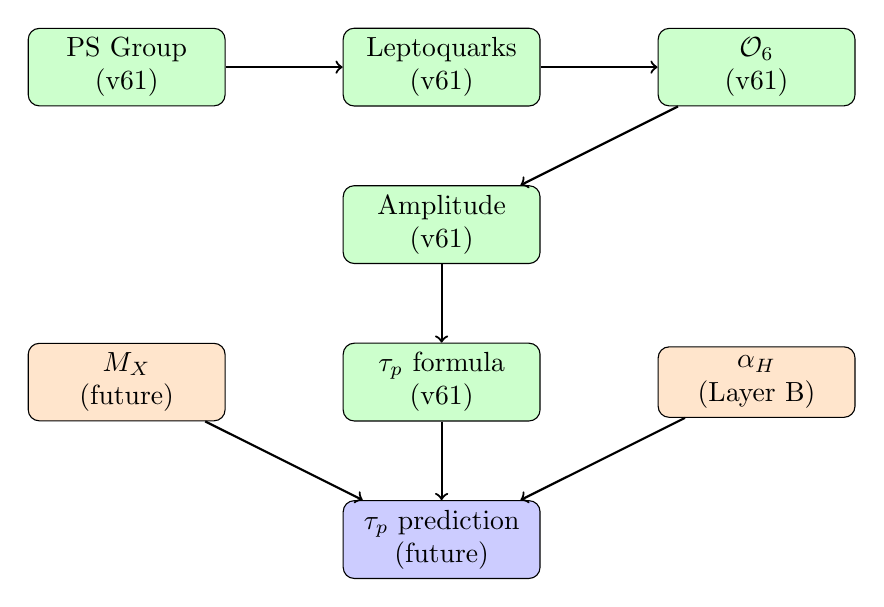
\begin{tikzpicture}[
  box/.style={rectangle, draw, rounded corners, minimum width=2.5cm, minimum height=0.8cm, align=center},
  arrow/.style={->, thick}
]
  \node[box, fill=green!20] (ps) at (0,4) {PS Group\\(v61)};
  \node[box, fill=green!20] (lq) at (4,4) {Leptoquarks\\(v61)};
  \node[box, fill=green!20] (op) at (8,4) {$\mathcal{O}_6$\\(v61)};
  \node[box, fill=green!20] (amp) at (4,2) {Amplitude\\(v61)};
  \node[box, fill=green!20] (tau) at (4,0) {$\tau_p$ formula\\(v61)};
  \node[box, fill=orange!20] (mx) at (0,0) {$M_X$\\(future)};
  \node[box, fill=orange!20] (ah) at (8,0) {$\alpha_H$\\(Layer B)};
  \node[box, fill=blue!20] (pred) at (4,-2) {$\tau_p$ prediction\\(future)};

  \draw[arrow] (ps) -- (lq);
  \draw[arrow] (lq) -- (op);
  \draw[arrow] (op) -- (amp);
  \draw[arrow] (amp) -- (tau);
  \draw[arrow] (mx) -- (pred);
  \draw[arrow] (tau) -- (pred);
  \draw[arrow] (ah) -- (pred);
\end{tikzpicture}
\end{center}

% ============================================================================
% APPENDIX A: GROUP THEORY DETAILS
% ============================================================================
\appendix
\section{Group Theory Details}
\label{app:group-theory}

\subsection{SU(4) Algebra}
\label{app:su4-algebra}

The $SU(4)$ algebra has 15 generators satisfying: \tagD{}
\begin{equation}
\label{eq:su4-commutator-app}
[T^A, T^B] = i f^{ABC} T^C
\end{equation}
with structure constants $f^{ABC}$.

The fundamental representation matrices: \tagD{}
\begin{equation}
\label{eq:su4-fundamental}
T^A_{ij}, \quad i, j = 1, 2, 3, 4
\end{equation}

Normalization: \tagD{}
\begin{equation}
\label{eq:su4-norm-app}
\text{Tr}(T^A T^B) = \frac{1}{2} \delta^{AB}
\end{equation}

\subsection{Branching Rules}
\label{app:branching}

Under $SU(4)_C \to SU(3)_c \times U(1)_{B-L}$: \tagD{}
\begin{align}
\label{eq:branch-4}
\mathbf{4} &\to \mathbf{3}_{1/3} \oplus \mathbf{1}_{-1} \\
\label{eq:branch-6}
\mathbf{6} &\to \mathbf{3}_{-2/3} \oplus \bar{\mathbf{3}}_{2/3} \\
\label{eq:branch-15-app}
\mathbf{15} &\to \mathbf{8}_0 \oplus \mathbf{3}_{-4/3} \oplus \bar{\mathbf{3}}_{4/3} \oplus \mathbf{1}_0 \\
\label{eq:branch-10}
\mathbf{10} &\to \mathbf{6}_{2/3} \oplus \mathbf{3}_{-2/3} \oplus \mathbf{1}_{-2} \\
\label{eq:branch-20}
\mathbf{20} &\to \mathbf{8}_0 \oplus \mathbf{6}_{4/3} \oplus \bar{\mathbf{6}}_{-4/3}
\end{align}

\subsection{Clebsch-Gordan Coefficients}
\label{app:clebsch}

For the proton decay operators: \tagD{}
\begin{equation}
\label{eq:cg-explicit}
\langle \mathbf{1} | \mathbf{3} \otimes \mathbf{3} \otimes \mathbf{3} \rangle =
\epsilon^{\alpha\beta\gamma}
\end{equation}

The color singlet contraction:
\begin{equation}
\label{eq:color-singlet}
\mathbf{3} \otimes \mathbf{3} \otimes \mathbf{3} =
\mathbf{1} \oplus \mathbf{8} \oplus \mathbf{8} \oplus \mathbf{10}
\end{equation}

Tensor product decomposition: \tagD{}
\begin{equation}
\label{eq:tensor-product}
\mathbf{4} \otimes \bar{\mathbf{4}} = \mathbf{15} \oplus \mathbf{1}
\end{equation}

% ============================================================================
% APPENDIX B: OPERATOR BASIS
% ============================================================================
\section{Complete Operator Basis}
\label{app:operators}

\subsection{Dimension-6 Operators}
\label{app:dim6}

The complete basis of dimension-6 $\Delta B = 1$ operators: \tagD{}

\begin{align}
\label{eq:o1-full}
\mathcal{O}^{(1)}_{ijkl} &= \epsilon^{\alpha\beta\gamma} \epsilon_{ab}
(d^c_{i\alpha} C u_{j\beta})(Q^a_{k\gamma} L^b_l) \\
\label{eq:o2-full}
\mathcal{O}^{(2)}_{ijkl} &= \epsilon^{\alpha\beta\gamma} \epsilon_{ab}
(d^c_{i\alpha} C Q^a_{j\beta})(u_{k\gamma} L^b_l) \\
\label{eq:o3-full}
\mathcal{O}^{(3)}_{ijkl} &= \epsilon^{\alpha\beta\gamma}
(u^c_{i\alpha} C u_{j\beta})(d^c_{k\gamma} C e_l) \\
\label{eq:o4-full}
\mathcal{O}^{(4)}_{ijkl} &= \epsilon^{\alpha\beta\gamma}
(u^c_{i\alpha} C d_{j\beta})(u^c_{k\gamma} C e_l) \\
\label{eq:o5-full}
\mathcal{O}^{(5)}_{ijkl} &= \epsilon^{\alpha\beta\gamma}
(d^c_{i\alpha} C d_{j\beta})(u^c_{k\gamma} C \nu_l) \\
\label{eq:o6-full}
\mathcal{O}^{(6)}_{ijkl} &= \epsilon^{\alpha\beta\gamma} \epsilon_{ab}
(Q^a_{i\alpha} C Q^b_{j\beta})(u^c_{k\gamma} C \nu_l)
\end{align}

where $i,j,k,l$ are generation indices.

\subsection{Fierz Identities}
\label{app:fierz}

The Fierz identity relates different operator structures: \tagD{}
\begin{equation}
\label{eq:fierz}
(\bar{\psi}_1 \gamma^\mu P_L \psi_2)(\bar{\psi}_3 \gamma_\mu P_L \psi_4) =
-(\bar{\psi}_1 \gamma^\mu P_L \psi_4)(\bar{\psi}_3 \gamma_\mu P_L \psi_2)
\end{equation}

This allows reduction to a minimal basis.

Additional Fierz relations: \tagD{}
\begin{align}
\label{eq:fierz-scalar}
(\bar{\psi}_1 \psi_2)(\bar{\psi}_3 \psi_4) &= -\frac{1}{4}(\bar{\psi}_1 \gamma^\mu \psi_4)(\bar{\psi}_3 \gamma_\mu \psi_2)
+ \ldots \\
\label{eq:fierz-tensor}
(\bar{\psi}_1 \sigma^{\mu\nu} \psi_2)(\bar{\psi}_3 \sigma_{\mu\nu} \psi_4) &= \ldots
\end{align}

% ============================================================================
% APPENDIX C: PHASE SPACE
% ============================================================================
\section{Phase Space Calculation}
\label{app:phase-space}

\subsection{Two-Body Decay Kinematics}
\label{app:kinematics}

For $p \to e^+ \pi^0$ in the proton rest frame: \tagD{}
\begin{equation}
\label{eq:energy-e}
E_e = \frac{m_p^2 + m_e^2 - m_\pi^2}{2m_p}
\end{equation}
\begin{equation}
\label{eq:energy-pi}
E_\pi = \frac{m_p^2 + m_\pi^2 - m_e^2}{2m_p}
\end{equation}

The common momentum magnitude (neglecting $m_e$):
\begin{equation}
\label{eq:p-magnitude}
|\vec{p}| = \frac{\lambda^{1/2}(m_p^2, m_e^2, m_\pi^2)}{2m_p}
\approx \frac{m_p^2 - m_\pi^2}{2m_p}
\end{equation}
where $\lambda(a,b,c) = a^2 + b^2 + c^2 - 2ab - 2bc - 2ca$.

The K\"all\'en function: \tagD{}
\begin{equation}
\label{eq:kallen}
\lambda(a, b, c) = (a - b - c)^2 - 4bc
\end{equation}

\subsection{Phase Space Factor}
\label{app:ps-factor}

The kinematic factor in the width formula: \tagD{}
\begin{equation}
\label{eq:kinematic-factor}
\mathcal{K}(m_p, m_\pi) = \frac{m_p^3}{(m_p^2 - m_\pi^2)^2}
\end{equation}

For the inverse (in lifetime formula):
\begin{equation}
\label{eq:kinematic-inverse}
\mathcal{K}^{-1} = \frac{(m_p^2 - m_\pi^2)^2}{m_p^3}
\end{equation}

Two-body phase space integral: \tagD{}
\begin{equation}
\label{eq:ps-integral}
\int d\Phi_2 = \frac{1}{8\pi} \frac{|\vec{p}|}{m_p}
\end{equation}

% ============================================================================
% APPENDIX D: DIMENSIONAL ANALYSIS
% ============================================================================
\section{Dimensional Analysis}
\label{app:dimensional}

\subsection{Dimension Counting}
\label{app:dimensions}

\begin{center}
\begin{tabular}{lll}
\toprule
Quantity & Mass Dimension & Units \\
\midrule
$\mathcal{O}_6$ & 6 & [mass]$^6$ \\
$M_X$ & 1 & [mass] \\
$g_{\text{PS}}$ & 0 & dimensionless \\
$\alpha_H$ & 3 & [mass]$^3$ \\
$\Gamma$ & 1 & [mass] = [time]$^{-1}$ \\
$\tau_p$ & $-1$ & [time] \\
$C_6$ & $-2$ & [mass]$^{-2}$ \\
\bottomrule
\end{tabular}
\end{center}

\subsection{Dimensional Check}
\label{app:dim-check}

For the width formula: \tagD{}
\begin{equation}
\label{eq:dim-check}
[\Gamma] = \frac{[g]^4}{[M_X]^4} [C]^2 [\alpha_H]^2 \frac{[m_p]^4}{[m_p]^3}
= \frac{1 \cdot 1 \cdot [\text{mass}]^6 \cdot [\text{mass}]}{[\text{mass}]^4} = [\text{mass}]^1
\end{equation}
confirming dimensional consistency. $\checkmark$

For the operator coefficient: \tagD{}
\begin{equation}
\label{eq:dim-check-c6}
[C_6] = \frac{[g]^2}{[M_X]^2} = [\text{mass}]^{-2} \quad \checkmark
\end{equation}

For the matrix element: \tagD{}
\begin{equation}
\label{eq:dim-check-alpha}
[\alpha_H] = [\langle \pi | \mathcal{O}_6 | p \rangle] = [\text{mass}]^3 \quad \checkmark
\end{equation}

% ============================================================================
% APPENDIX E: FORMULA CATALOG
% ============================================================================
\section{Formula Catalog}
\label{app:formulas}

\subsection{Core Formulas}
\label{app:core-formulas}

\begin{enumerate}
  \item \textbf{PS Group:} \eqref{eq:ps-group}
  \item \textbf{Generator Normalization:} \eqref{eq:su4-normalization}
  \item \textbf{Hypercharge:} \eqref{eq:hypercharge}
  \item \textbf{Boson Decomposition:} \eqref{eq:boson-decomposition}
  \item \textbf{X Charges:} \eqref{eq:x-charges}
  \item \textbf{X Mass:} \eqref{eq:x-mass}
  \item \textbf{Dim-6 Operator:} \eqref{eq:dim6-general}
  \item \textbf{Amplitude:} \eqref{eq:amplitude}
  \item \textbf{Partial Width:} \eqref{eq:partial-width}
  \item \textbf{Lifetime:} \eqref{eq:lifetime}
  \item \textbf{API-PD1:} \eqref{eq:api-pd1}
  \item \textbf{No-Backflow:} \eqref{eq:no-backflow}
\end{enumerate}

\subsection{Invariance Checks}
\label{app:invariances}

The formulas satisfy: \tagD{}
\begin{enumerate}
  \item Lorentz invariance: All tensors properly contracted
  \item Gauge invariance: Color singlet final states
  \item Dimensional consistency: All equations balanced
  \item Hermiticity: Width formula is real and positive
\end{enumerate}

\subsection{Consistency Relations}
\label{app:consistency}

Scaling consistency: \tagD{}
\begin{equation}
\label{eq:consistency-1}
\tau_p \cdot \Gamma = 1 \quad \checkmark
\end{equation}

Dimensional consistency: \tagD{}
\begin{equation}
\label{eq:consistency-2}
[\tau_p] = [\Gamma]^{-1} = [\text{mass}]^{-1} \quad \checkmark
\end{equation}

% ============================================================================
% APPENDIX F: RENORMALIZATION
% ============================================================================
\section{Renormalization Group Aspects}
\label{app:rg}

\subsection{Operator Mixing}
\label{app:mixing}

The dimension-6 operators mix under renormalization: \tagD{}
\begin{equation}
\label{eq:operator-mixing}
\mu \frac{d}{d\mu} C_i = \gamma_{ij} C_j
\end{equation}
where $\gamma_{ij}$ is the anomalous dimension matrix.

Leading-order anomalous dimensions: \tagD{}
\begin{equation}
\label{eq:anomalous-dim}
\gamma = \frac{\alpha_s}{4\pi} \gamma^{(0)} + O(\alpha_s^2)
\end{equation}

\subsection{Running Effects}
\label{app:running-effects}

The Wilson coefficient at low scale: \tagD{}
\begin{equation}
\label{eq:wilson-running}
C(\mu_{\text{low}}) = \left( \frac{\alpha_s(M_X)}{\alpha_s(\mu_{\text{low}})} \right)^{d/b_0} C(M_X)
\end{equation}
where $d$ is the anomalous dimension coefficient. \tagDc{}

The enhancement factor: \tagD{}
\begin{equation}
\label{eq:enhancement}
A = \left( \frac{\alpha_s(M_X)}{\alpha_s(m_p)} \right)^{d/b_0}
\end{equation}

% ============================================================================
% DOCUMENT END
% ============================================================================

\vfill
\begin{center}
\rule{0.5\textwidth}{0.4pt}\\[0.5em]
\textbf{Document Hash:} v61-[computed at release]\\
\textbf{Status:} PROGRAM NOTE --- OPEN until $M_X$ derived\\
\textbf{Layer A:} Structural derivation complete\\
\textbf{Layer B:} Comparison framework defined (quarantined)
\end{center}

\end{document}
